\section{Постановка задачи}
Для 5 распределений:
\begin{itemize}
\item нормальное распределение \( N(x, 0, 1) \)
\item распределение Коши \( C(x, 0, 1) \)
\item распределение Лапласа \( L(x, 0, 1/\sqrt{2}) \)
\item распределение Пуассона \( P(k, 10) \)
\item равномерное распределение \( U(x, -\sqrt{3}, \sqrt{3}) \)
\end{itemize}
Сгенерировать выборки размером 20, 60 и 100 элементов.
Построить на них эмпирические функции распределения и ядерные оценки плотности распределения на отрезке [−4; 4] для непрерывных распределений и на отрезке [6; 14] для распределения Пуассона.


\section{Теория}
\subsection{Эмпирическая функция распределения}
Эмпирическая функция распределения является оценкой генеральной функции распределения:
\[F_{n}^{*}(x) \approx F_{X}(x)\]
\\
Значения этой функции получаем так:
\[F_{n}^{*}(y) = \frac{1}{n} \sum_{i=1}^n I(X_i < y)\]
\[I(X_i < y) - \text{индикаторная функция}\]

\subsection{Ядерная оценка плотности вероятности}
Ядерная оценка плотности вероятности может быть найдена по формуле:
\[\hat{f_n}(x) = \frac{1}{nh_n} \sum_{i=1}^n K(\frac{x - x_i}{h_n})\]
Здесь функция \(K(y)\) - ядро, она может быть выбрана различными способами. Будем использовать Гауссово (нормальное) ядро:
\[K(y) = \frac{1}{\sqrt{2\pi}} \exp{-\frac{y^2}{2}}\]

Параметр сглаживания (диапазон частот) будем считать по правилу Сильвермана.


\section{Реализация}
\begin{itemize}
\item Язык: Python
\item Среда разработки: PyCharm
\item Используемые библиотеки: NumPy, SciPy, MatPlotLib, Seaborn
\end{itemize}


\section{Результаты}
\subsection{Эмпирические функции распределения}

\subsubsection{Нормальное распределение}
\begin{figure}[H]
	\begin{center}
		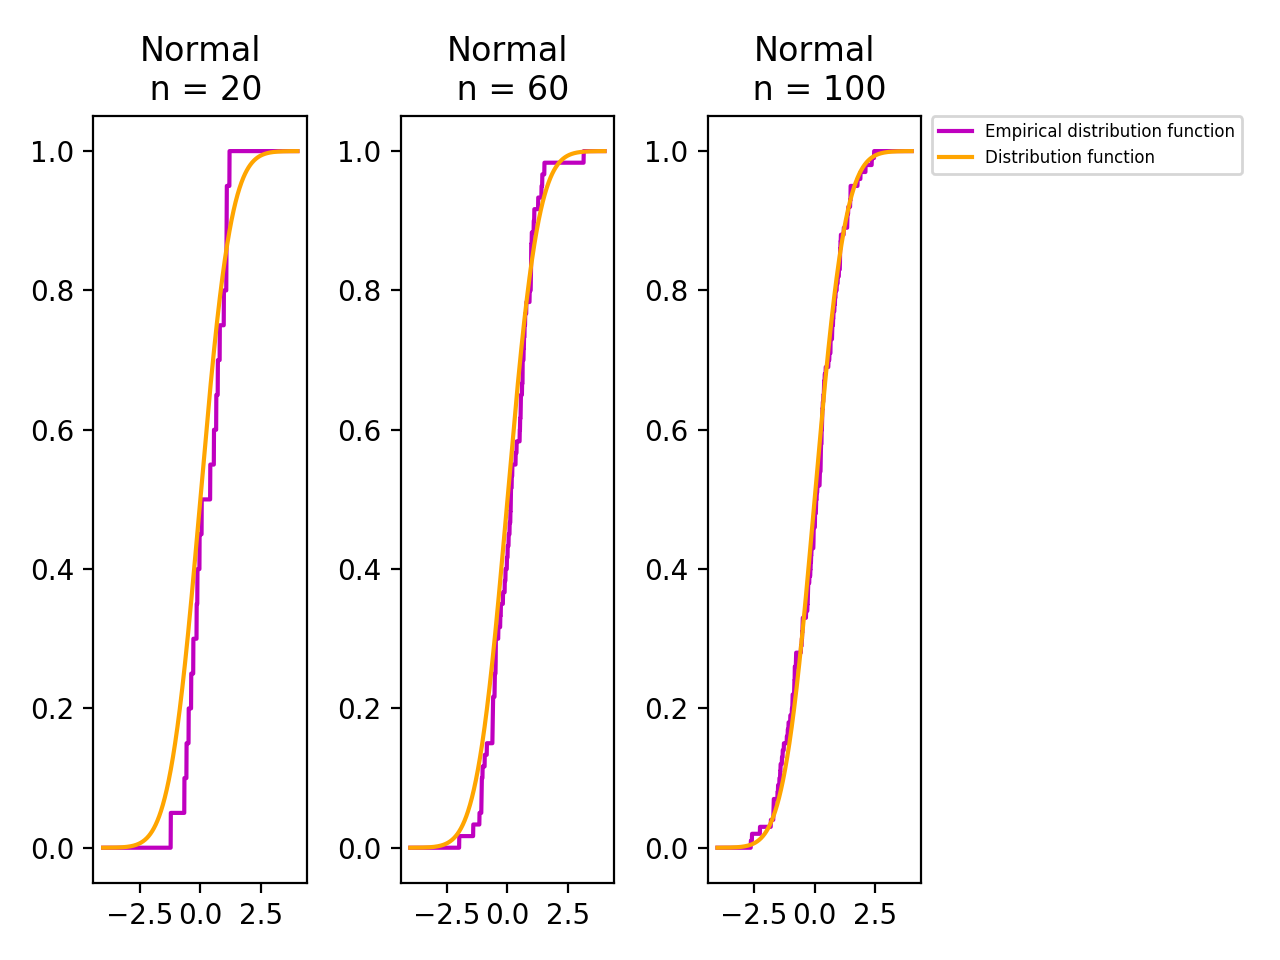
\includegraphics[scale=0.7]{fig/Normal_cde.png}
		\caption{Нормальное распределение} 
		\label{pic:pic_name}
	\end{center}
\end{figure}


\subsubsection{Распределение Коши}
\begin{figure}[H]
	\begin{center}
		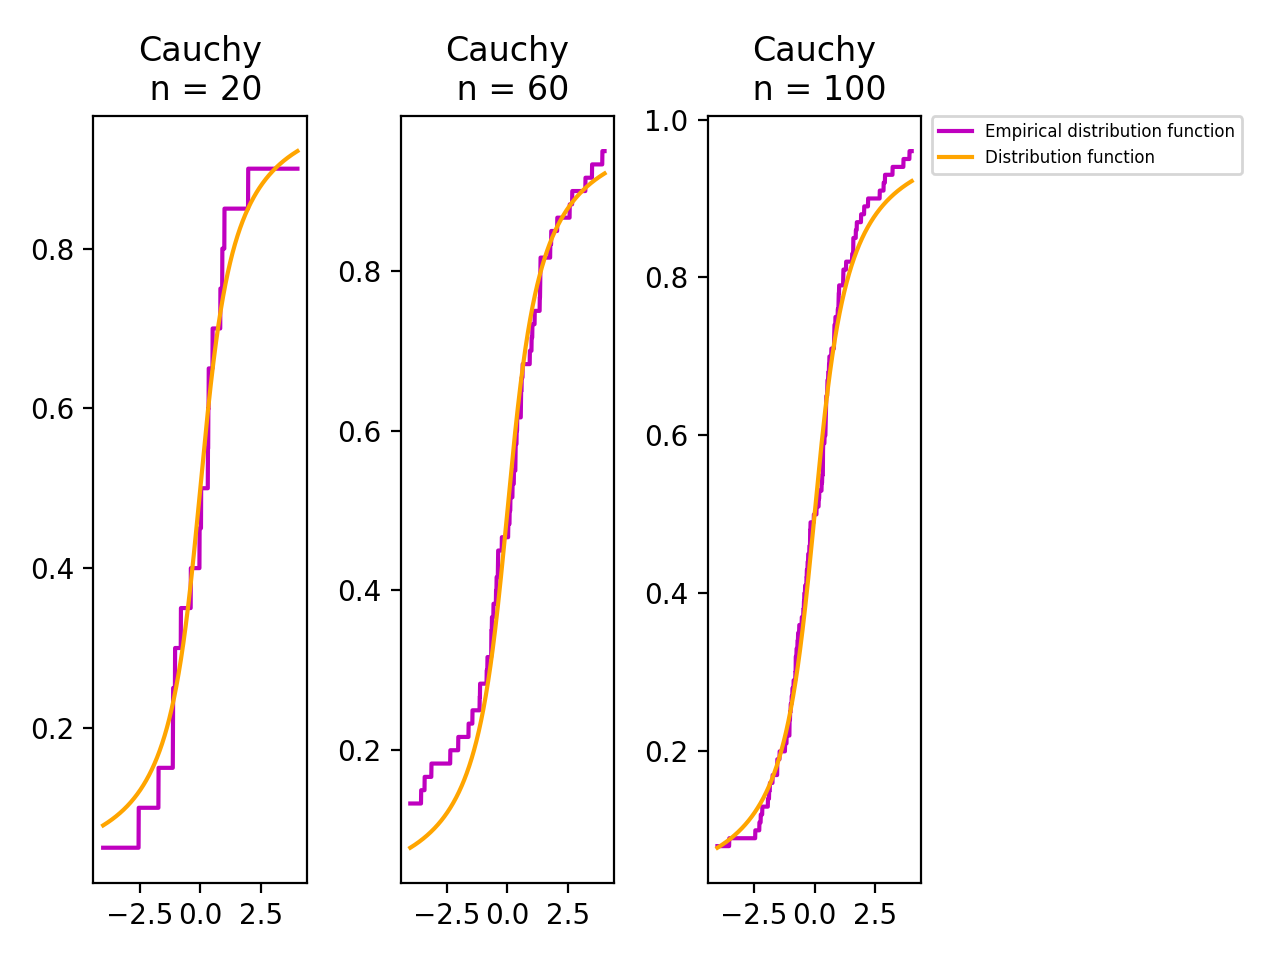
\includegraphics[scale=0.7]{fig/Cauchy_cde.png}
		\caption{Распределение Коши} 
		\label{pic:pic_name}
	\end{center}
\end{figure}


\subsubsection{Распределение Лапласа}
\begin{figure}[H]
	\begin{center}
		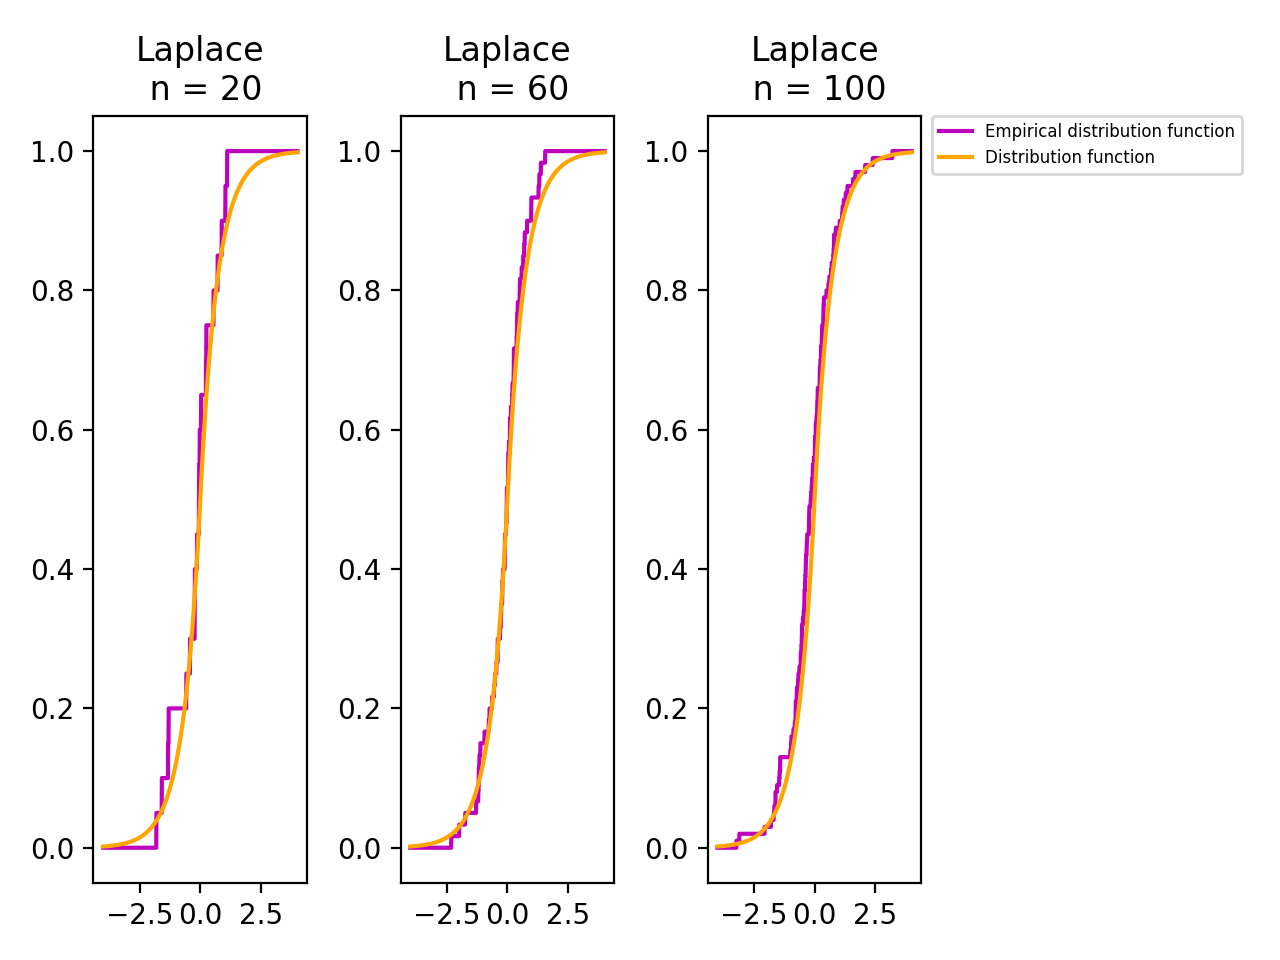
\includegraphics[scale=0.7]{fig/Laplace_cde.png}
		\caption{Распределение Лапласа} 
		\label{pic:pic_name}
	\end{center}
\end{figure}


\subsubsection{Распределение Пуассона}
\begin{figure}[H]
	\begin{center}
		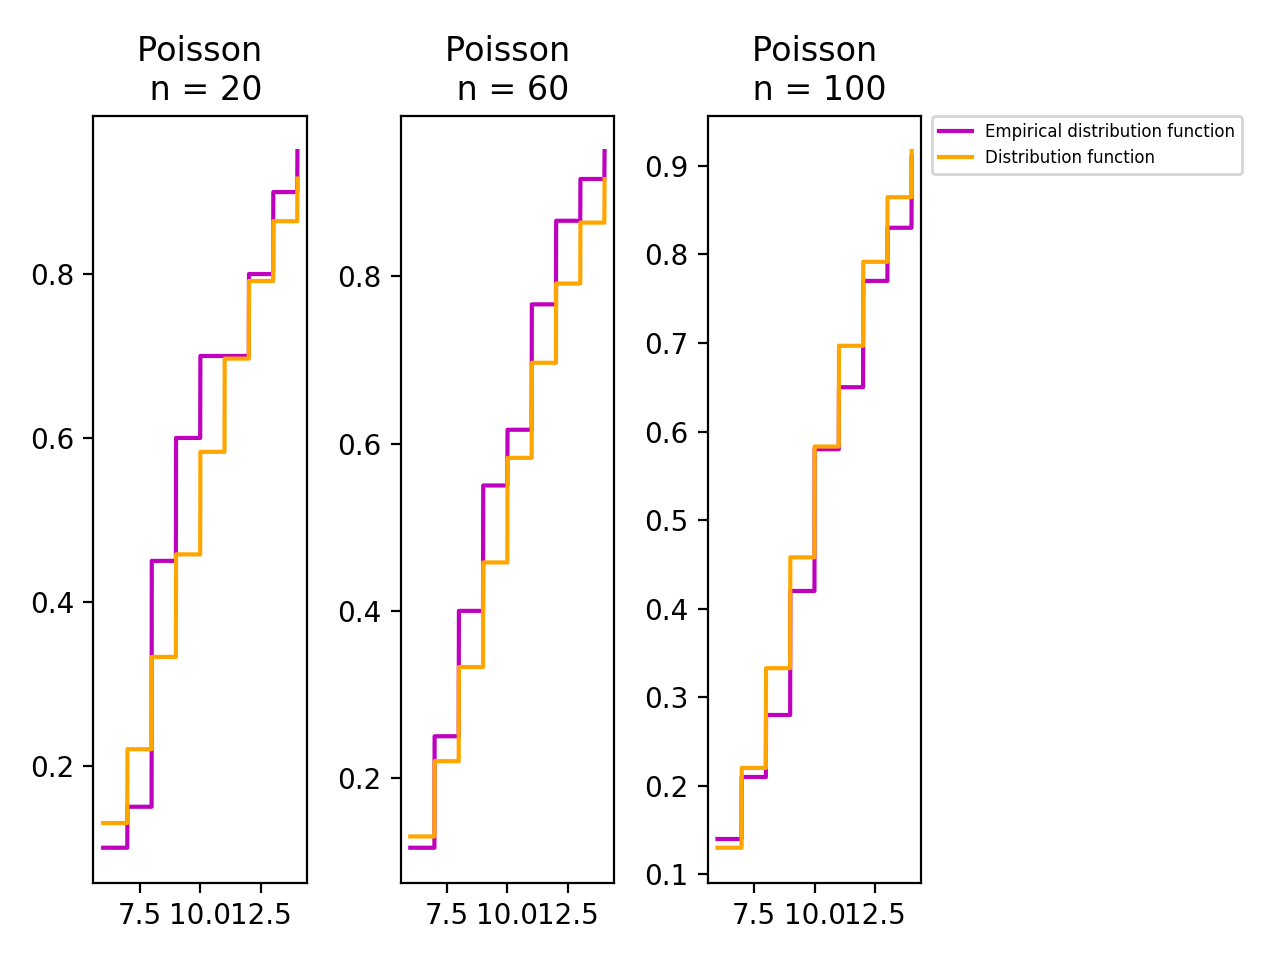
\includegraphics[scale=0.7]{fig/Poisson_cde.png}
		\caption{Распределение Пуассона} 
		\label{pic:pic_name} 
	\end{center}
\end{figure}


\subsubsection{Равномерное распределение}
\begin{figure}[H]
	\begin{center}
		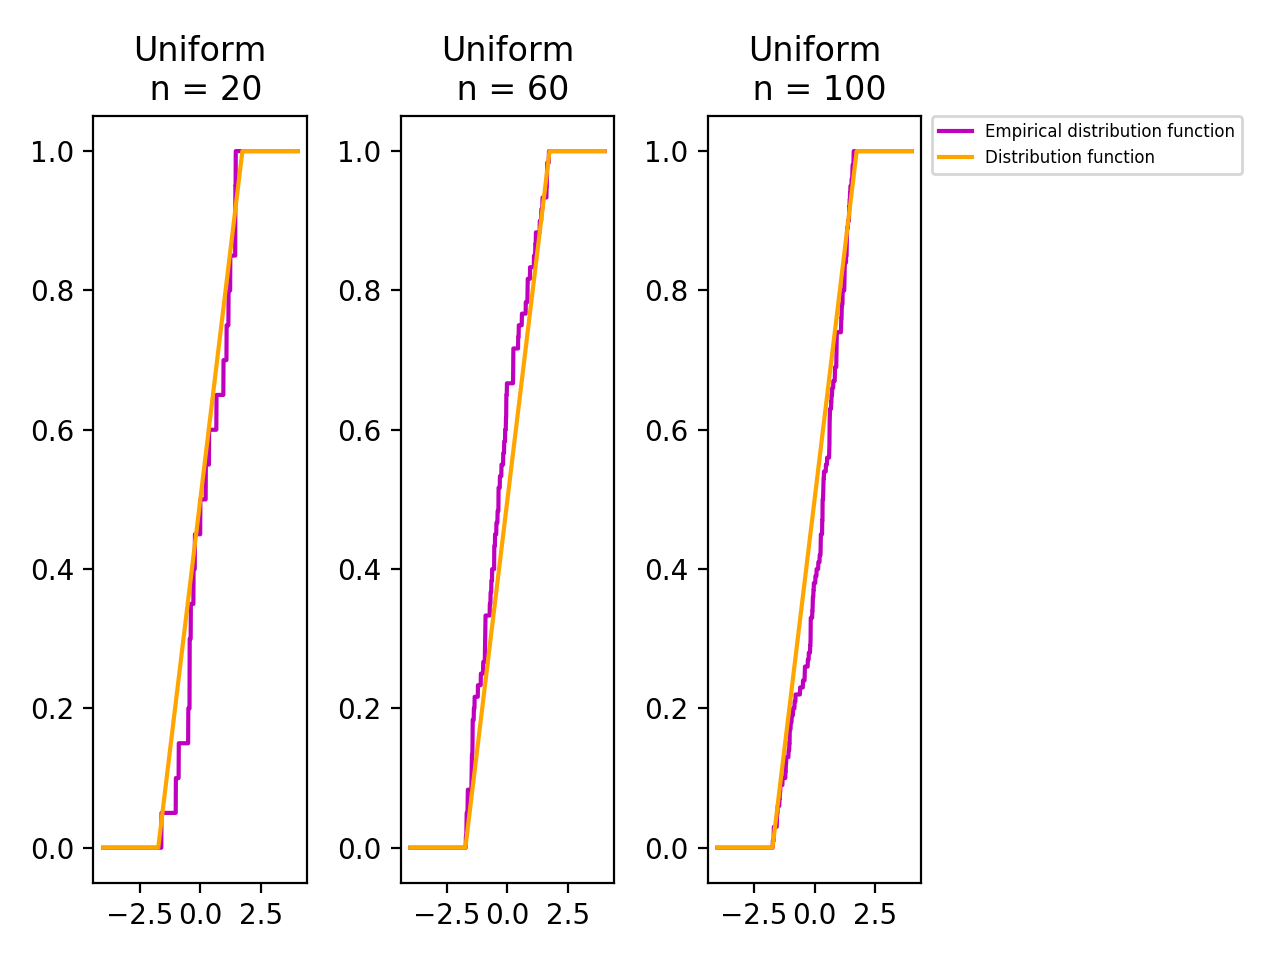
\includegraphics[scale=0.7]{fig/Uniform_cde.png}
		\caption{Равномерное распределение} 
		\label{pic:pic_name}
	\end{center}
\end{figure}



\subsection{Ядерные оценки плотности распределения}

\subsubsection{Нормальное распределение}
\begin{figure}[H]
	\begin{center}
		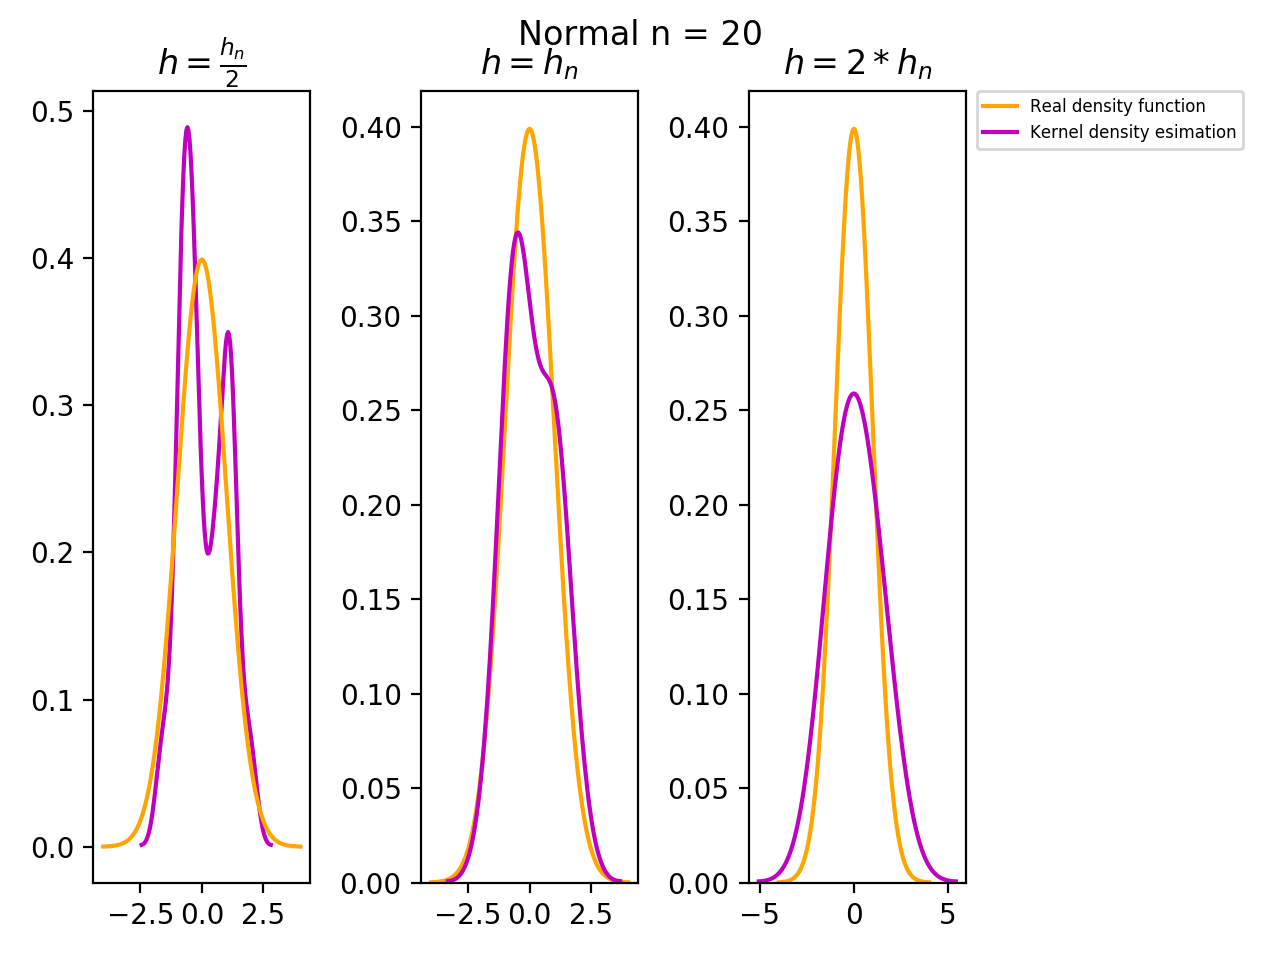
\includegraphics[scale=0.7]{fig/Normal20_kde.png}
		\caption{Нормальное распределение, n = 20} 
		\label{pic:pic_name}
	\end{center}
\end{figure}

\begin{figure}[H]
	\begin{center}
		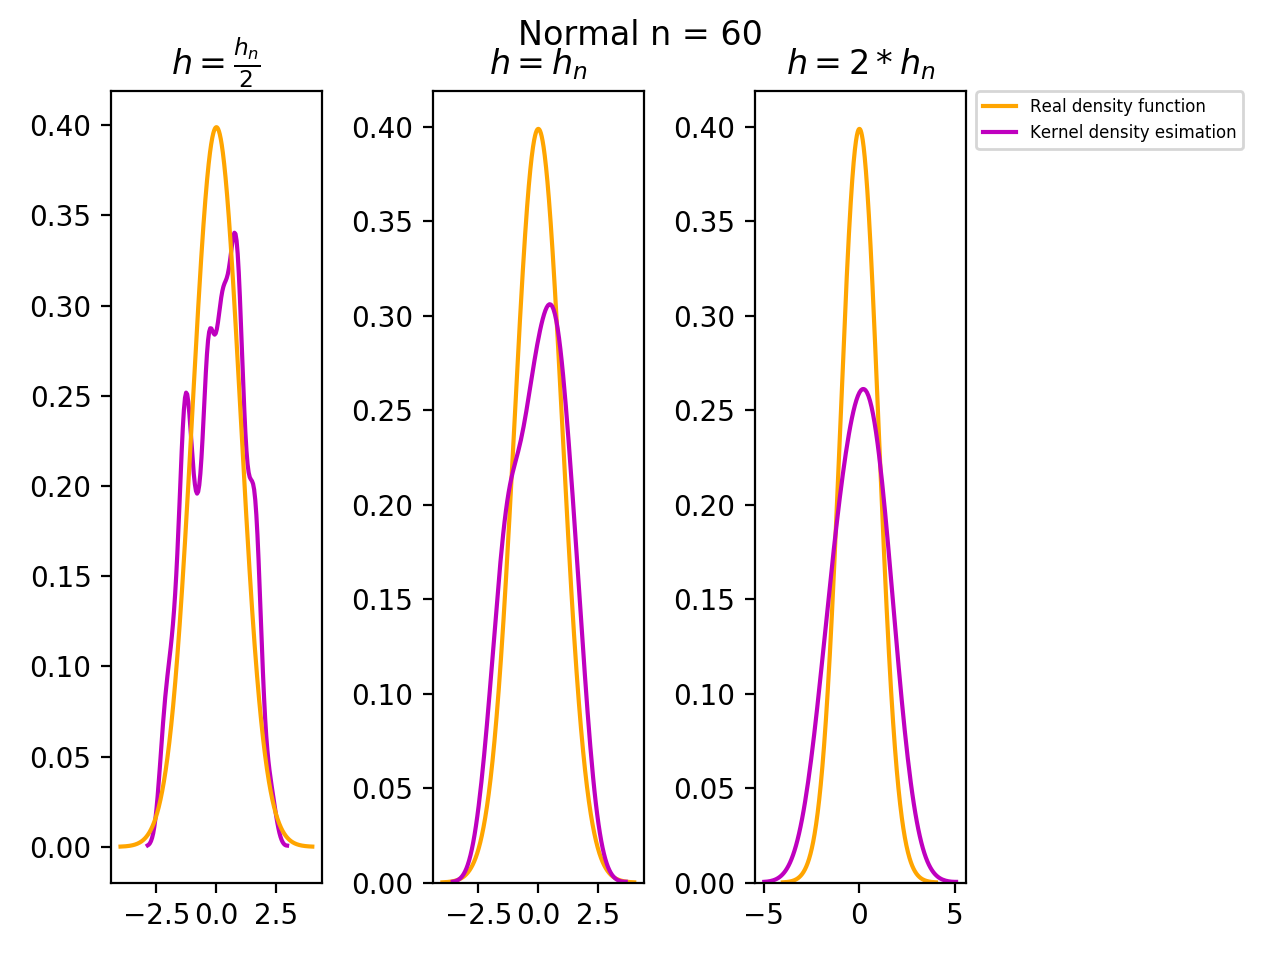
\includegraphics[scale=0.7]{fig/Normal60_kde.png}
		\caption{Нормальное распределение, n = 60} 
		\label{pic:pic_name}
	\end{center}
\end{figure}

\begin{figure}[H]
	\begin{center}
		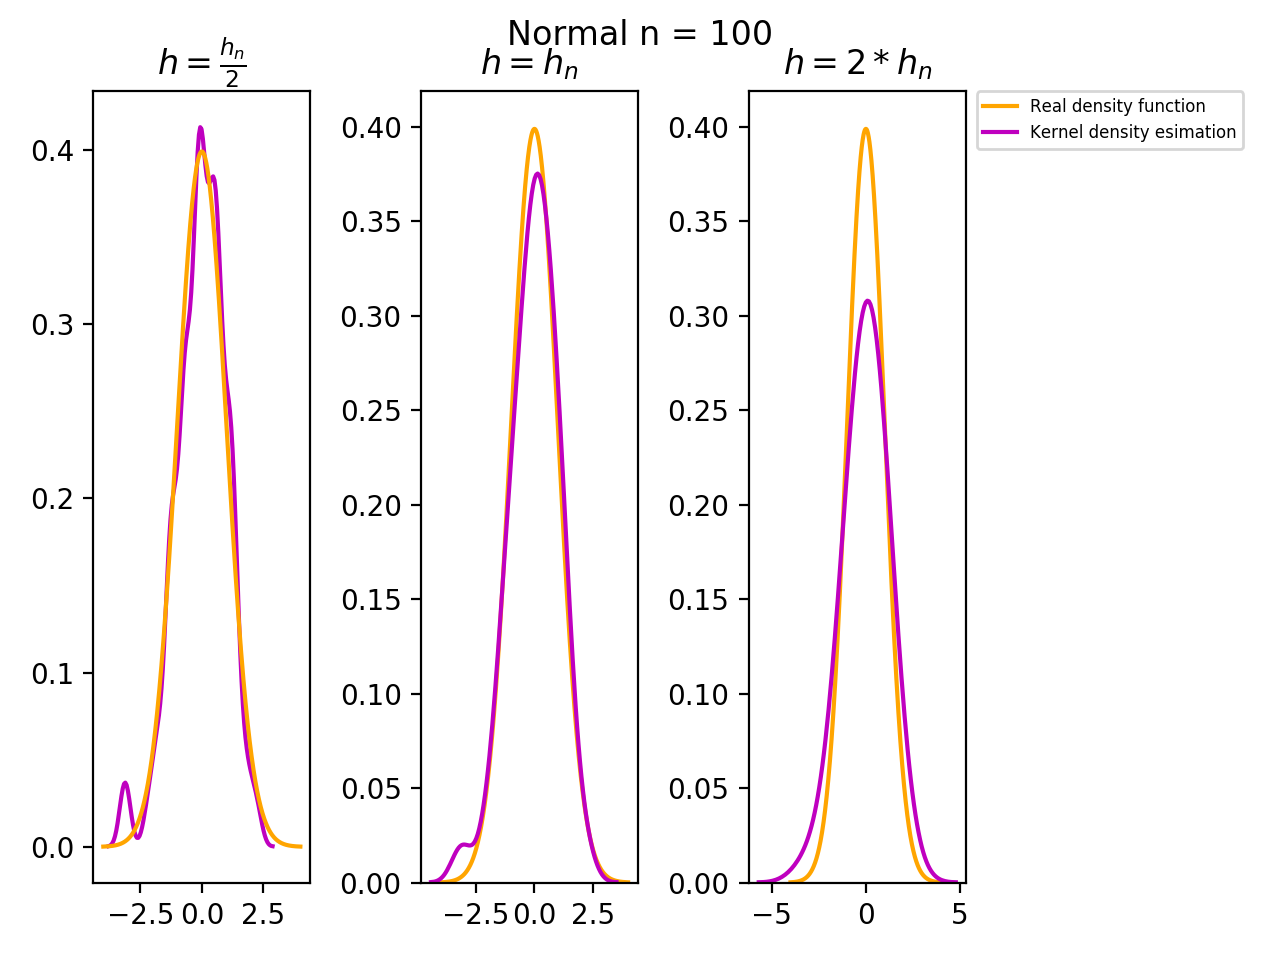
\includegraphics[scale=0.7]{fig/Normal100_kde.png}
		\caption{Нормальное распределение, n = 100} 
		\label{pic:pic_name}
	\end{center}
\end{figure}




\subsubsection{Распределение Коши}
\begin{figure}[H]
	\begin{center}
		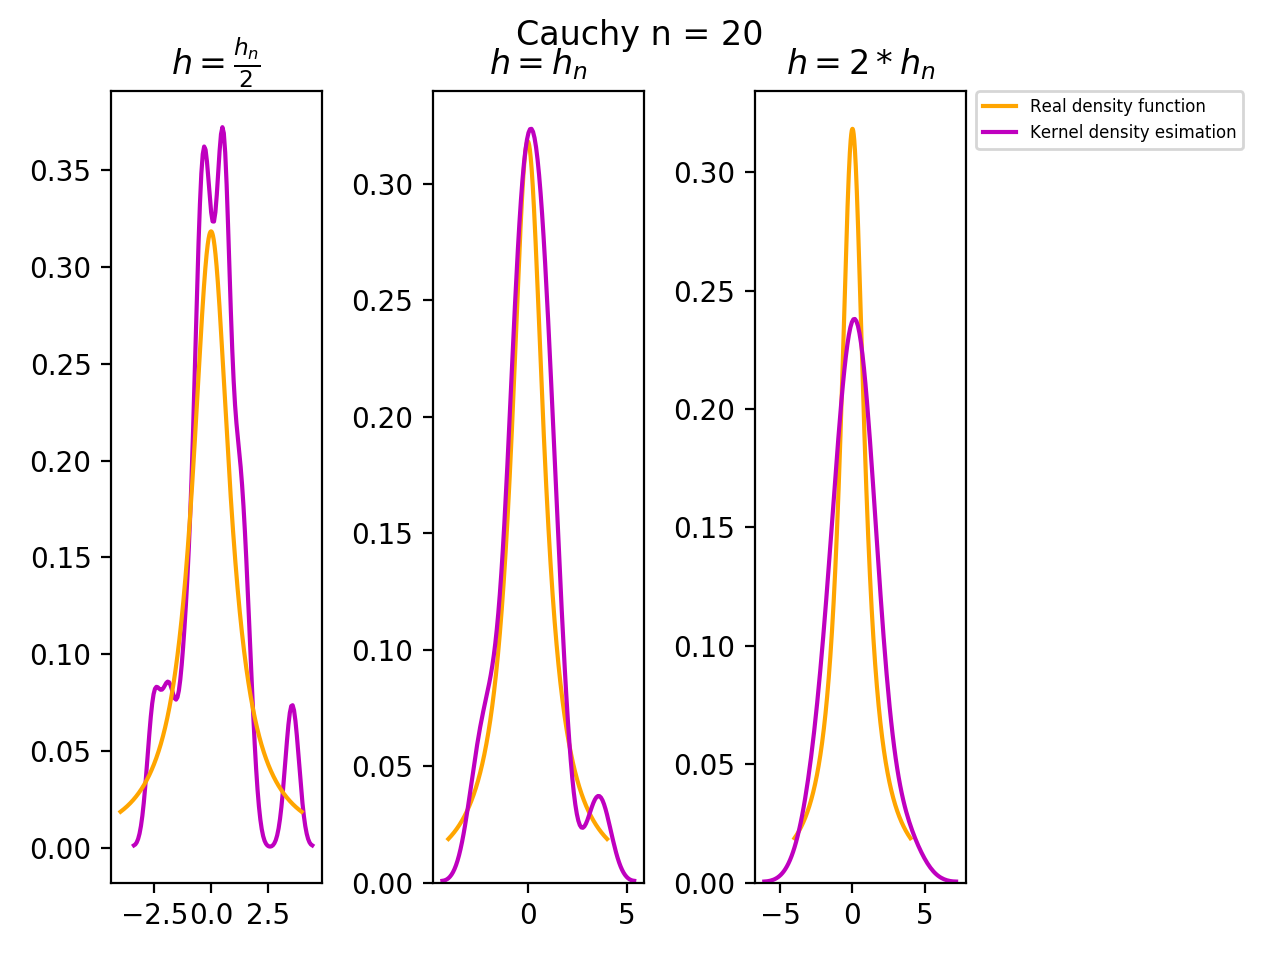
\includegraphics[scale=0.7]{fig/Cauchy20_kde.png}
		\caption{Распределение Коши, n = 20} 
		\label{pic:pic_name}
	\end{center}
\end{figure}

\begin{figure}[H]
	\begin{center}
		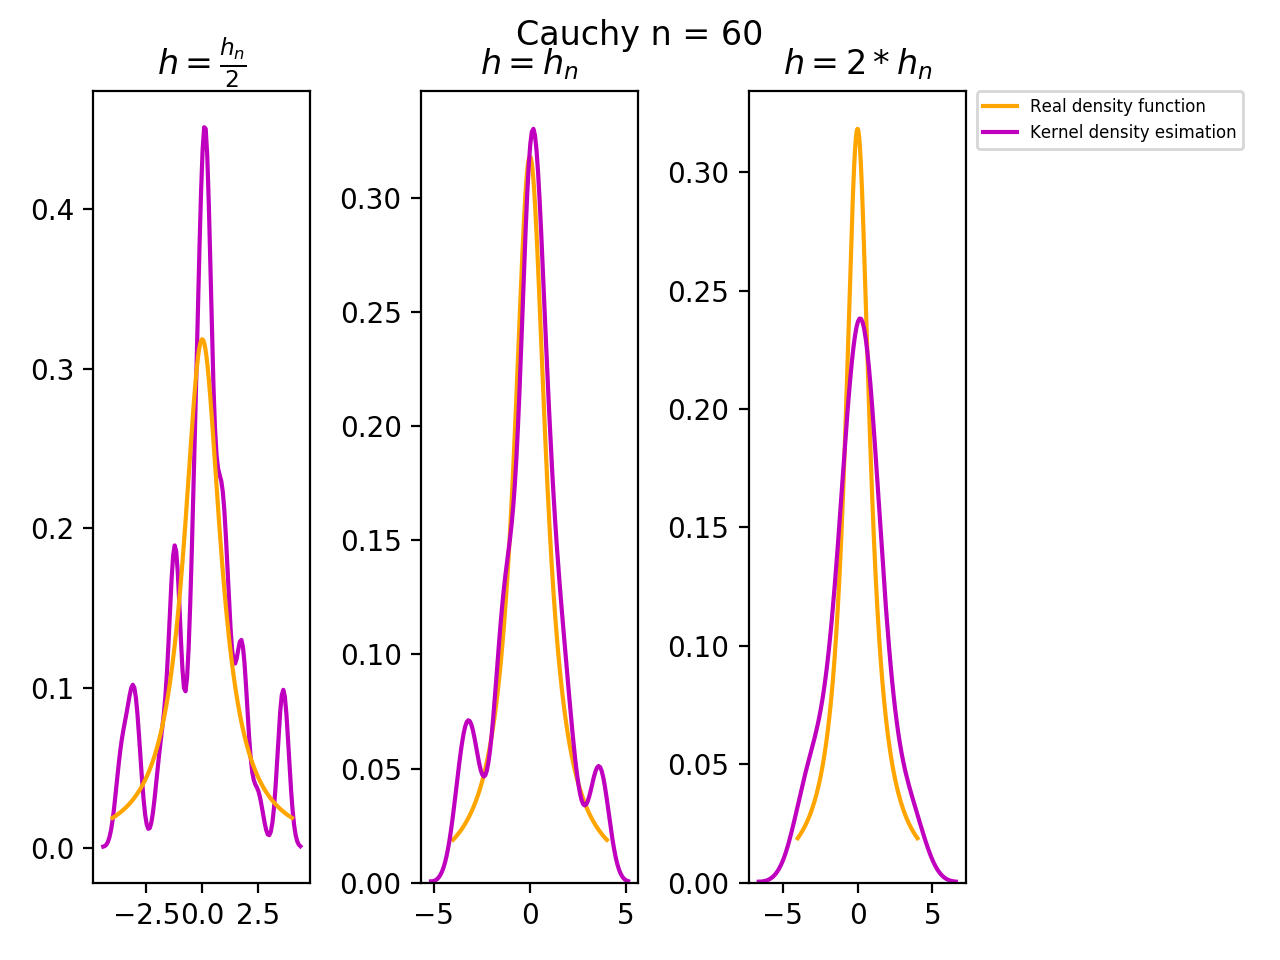
\includegraphics[scale=0.7]{fig/Cauchy60_kde.png}
		\caption{Распределение Коши, n = 60} 
		\label{pic:pic_name}
	\end{center}
\end{figure}

\begin{figure}[H]
	\begin{center}
		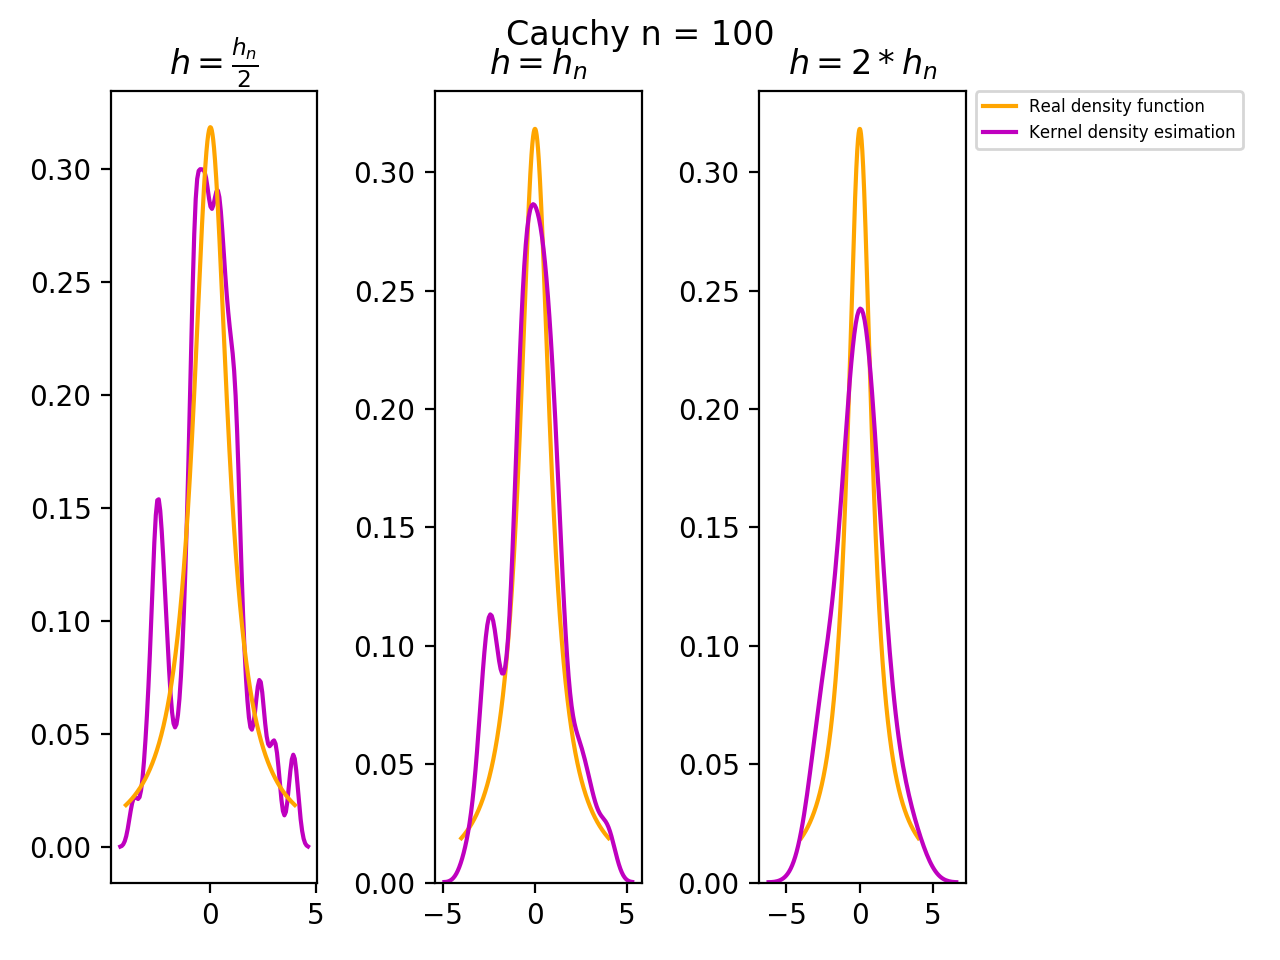
\includegraphics[scale=0.7]{fig/Cauchy100_kde.png}
		\caption{Распределение Коши, n = 100} 
		\label{pic:pic_name}
	\end{center}
\end{figure}

\subsubsection{Распределение Лапласа}
\begin{figure}[H]
	\begin{center}
		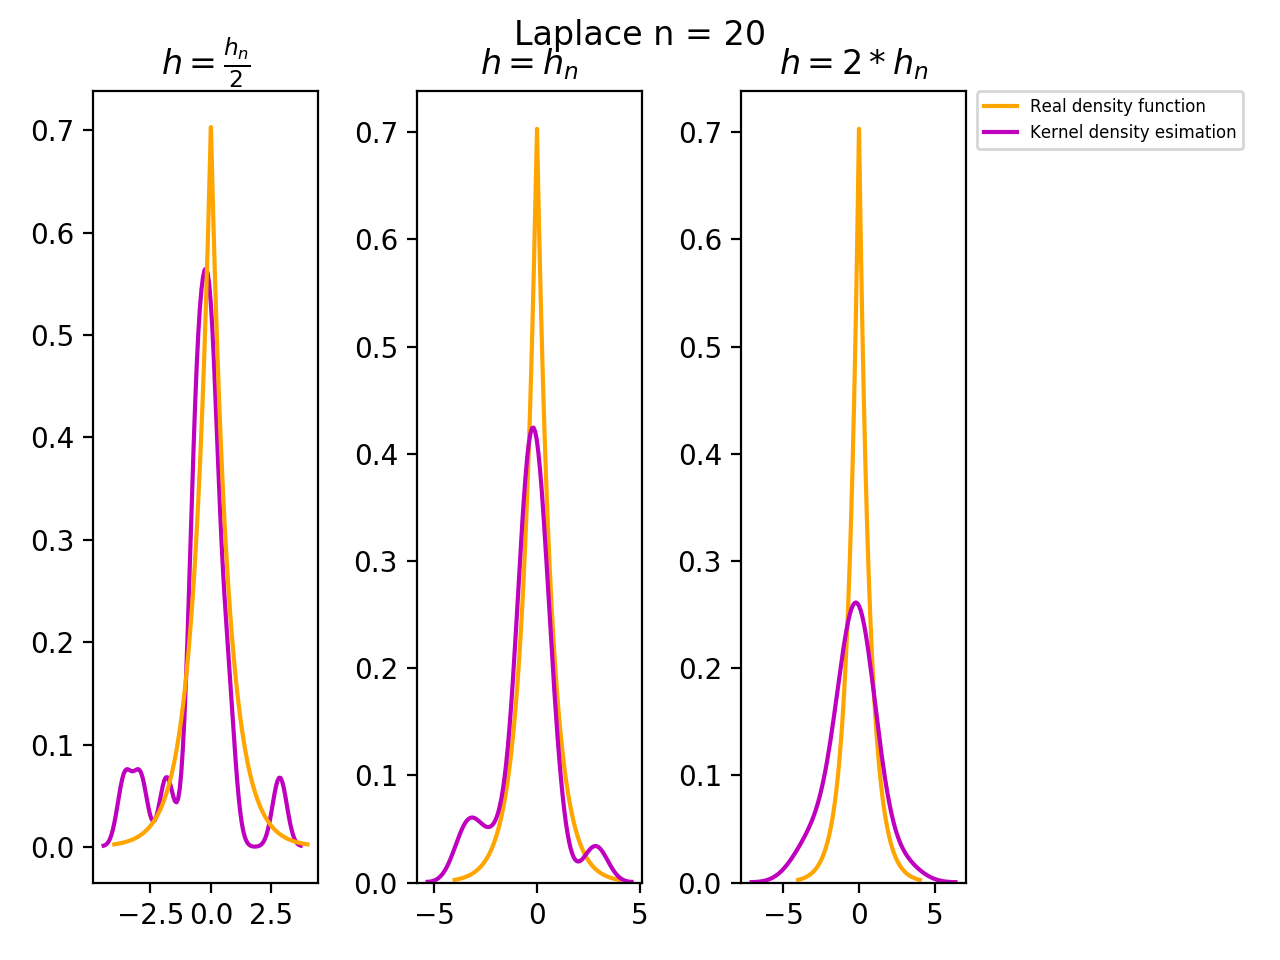
\includegraphics[scale=0.7]{fig/Laplace20_kde.png}
		\caption{Распределение Лапласа, n = 20} 
		\label{pic:pic_name}
	\end{center}
\end{figure}

\begin{figure}[H]
	\begin{center}
		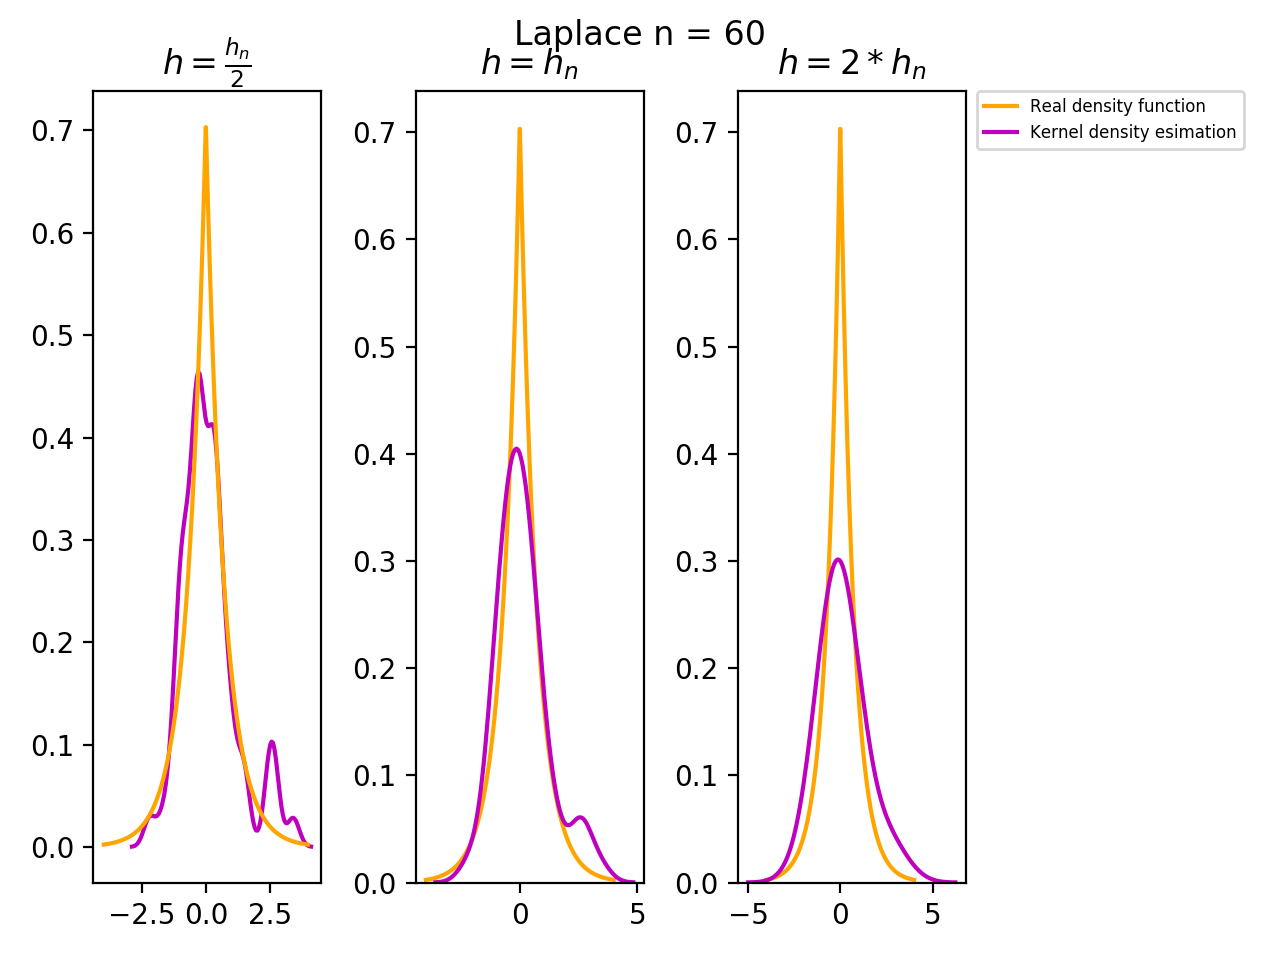
\includegraphics[scale=0.7]{fig/Laplace60_kde.png}
		\caption{Распределение Лапласа, n = 60} 
		\label{pic:pic_name}
	\end{center}
\end{figure}

\begin{figure}[H]
	\begin{center}
		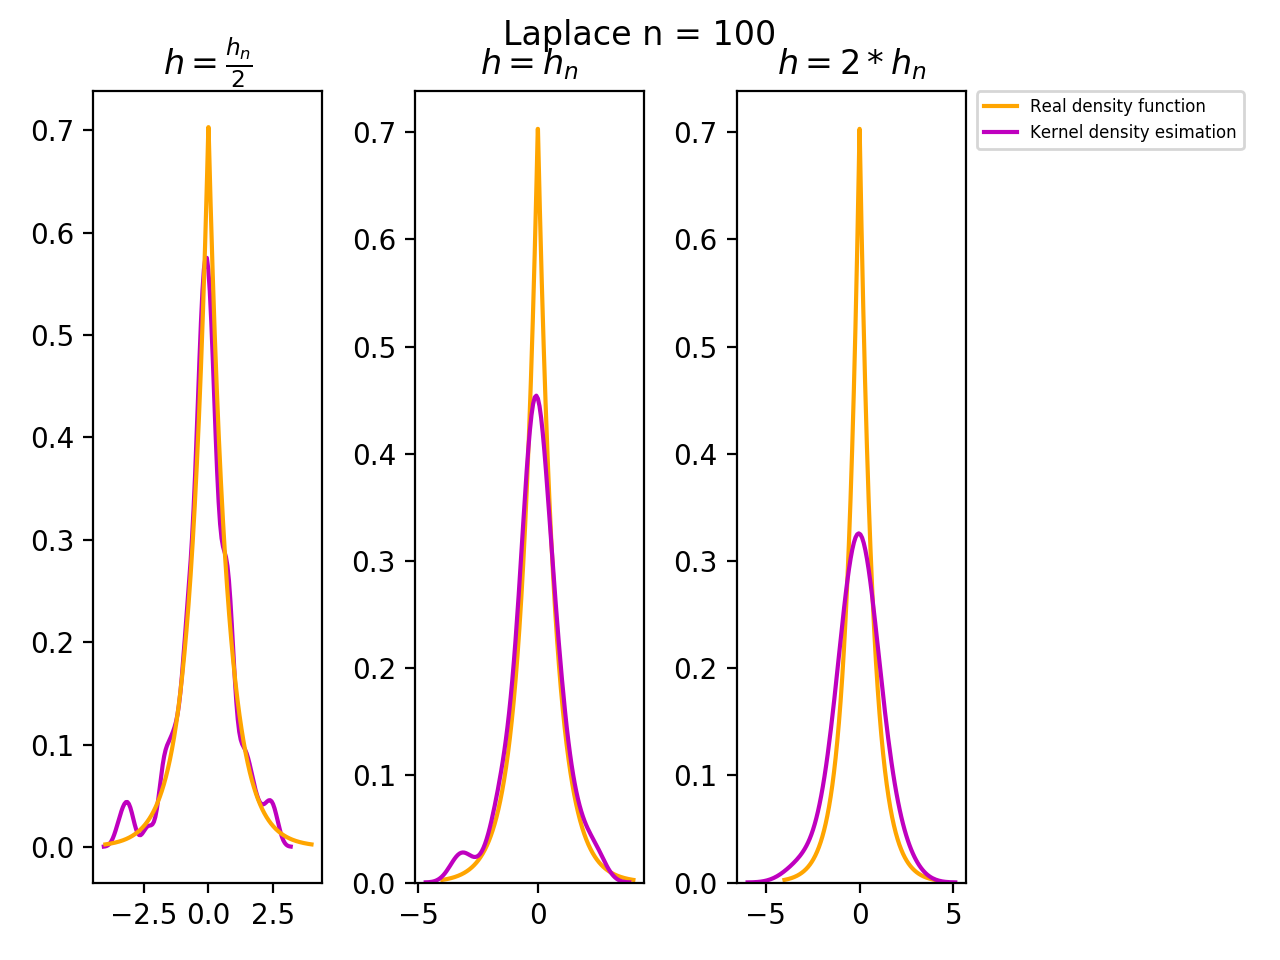
\includegraphics[scale=0.7]{fig/Laplace100_kde.png}
		\caption{Распределение Лапласа, n = 100} 
		\label{pic:pic_name}
	\end{center}
\end{figure}



\subsubsection{Распределение Пуассона}
\begin{figure}[H]
	\begin{center}
		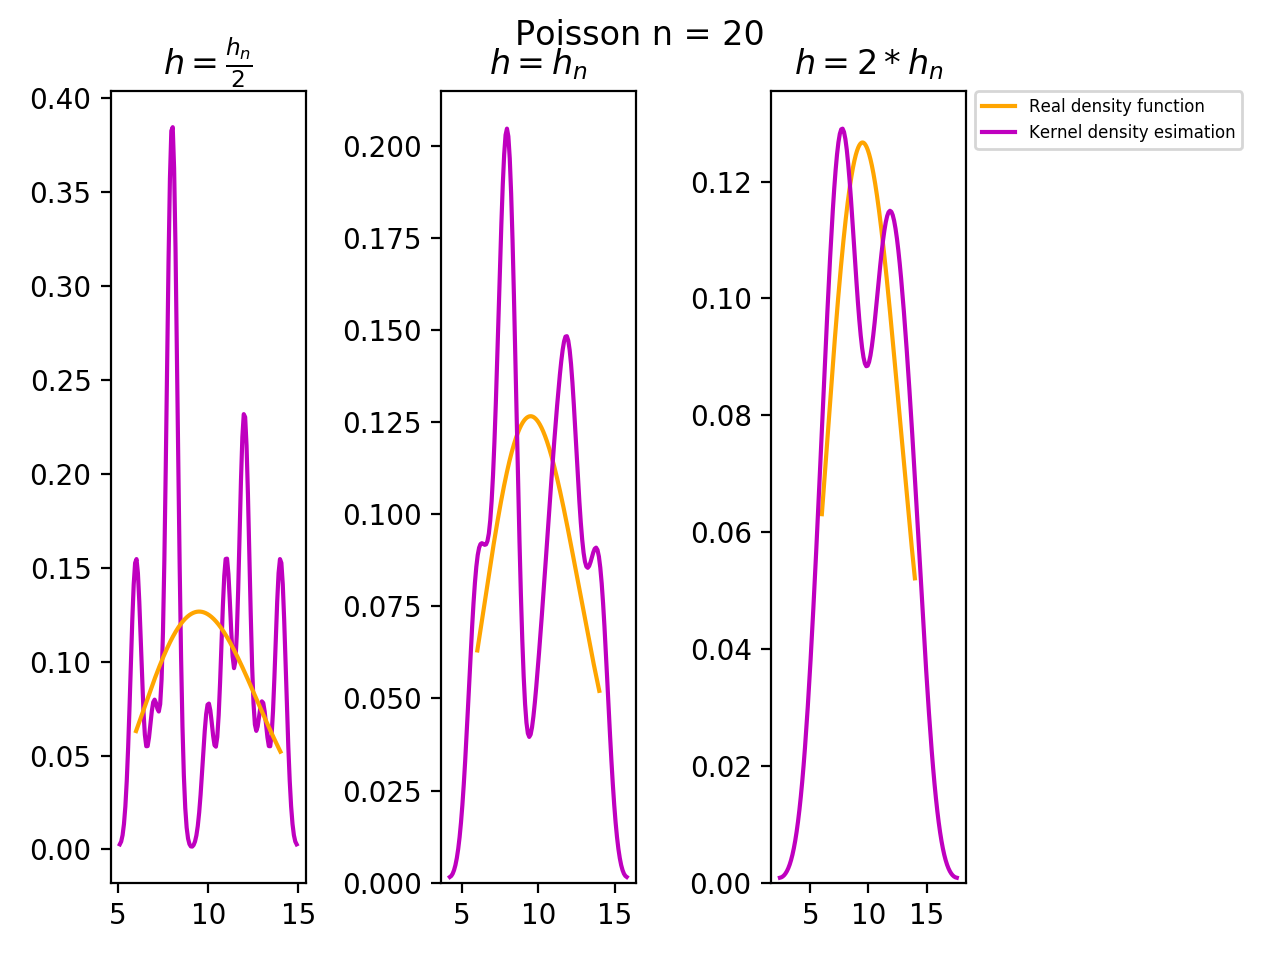
\includegraphics[scale=0.7]{fig/Poisson20_kde.png}
		\caption{Распределение Пуассона, n = 20} 
		\label{pic:pic_name} 
	\end{center}
\end{figure}

\begin{figure}[H]
	\begin{center}
		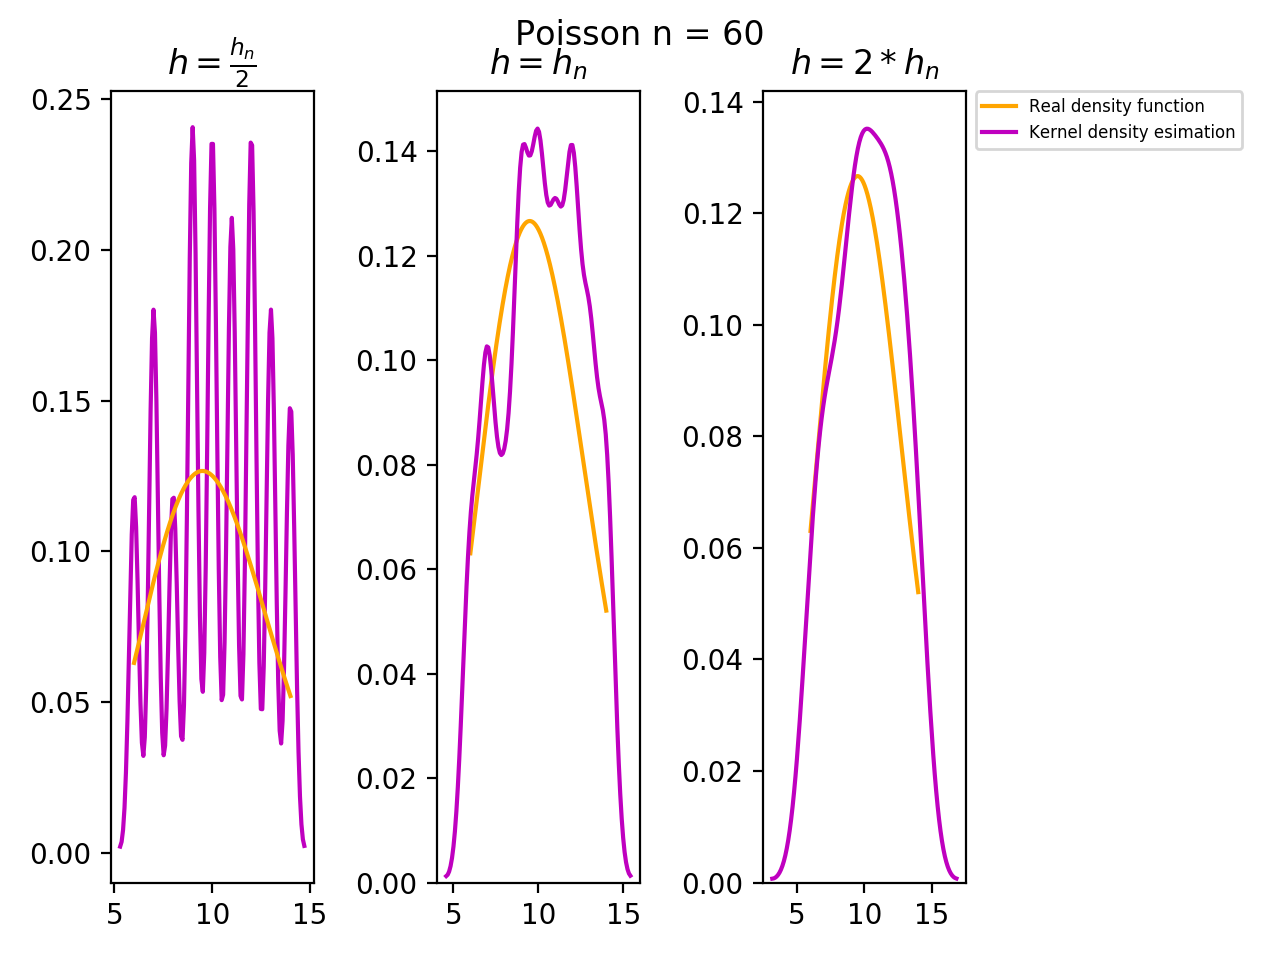
\includegraphics[scale=0.7]{fig/Poisson60_kde.png}
		\caption{Распределение Пуассона, n = 60} 
		\label{pic:pic_name} 
	\end{center}
\end{figure}

\begin{figure}[H]
	\begin{center}
		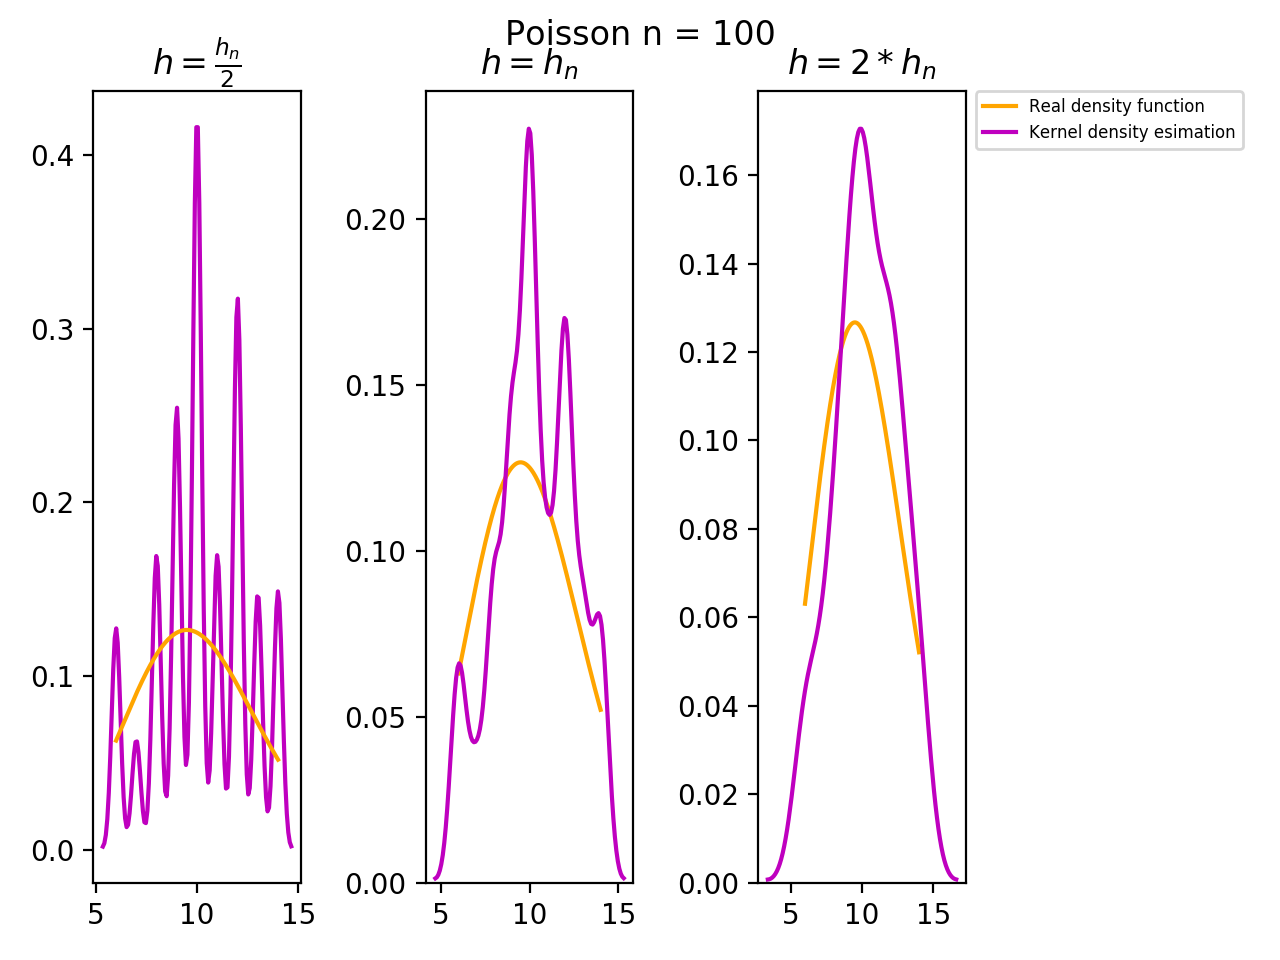
\includegraphics[scale=0.7]{fig/Poisson100_kde.png}
		\caption{Распределение Пуассона, n = 100} 
		\label{pic:pic_name} 
	\end{center}
\end{figure}


\subsubsection{Равномерное распределение}
\begin{figure}[H]
	\begin{center}
		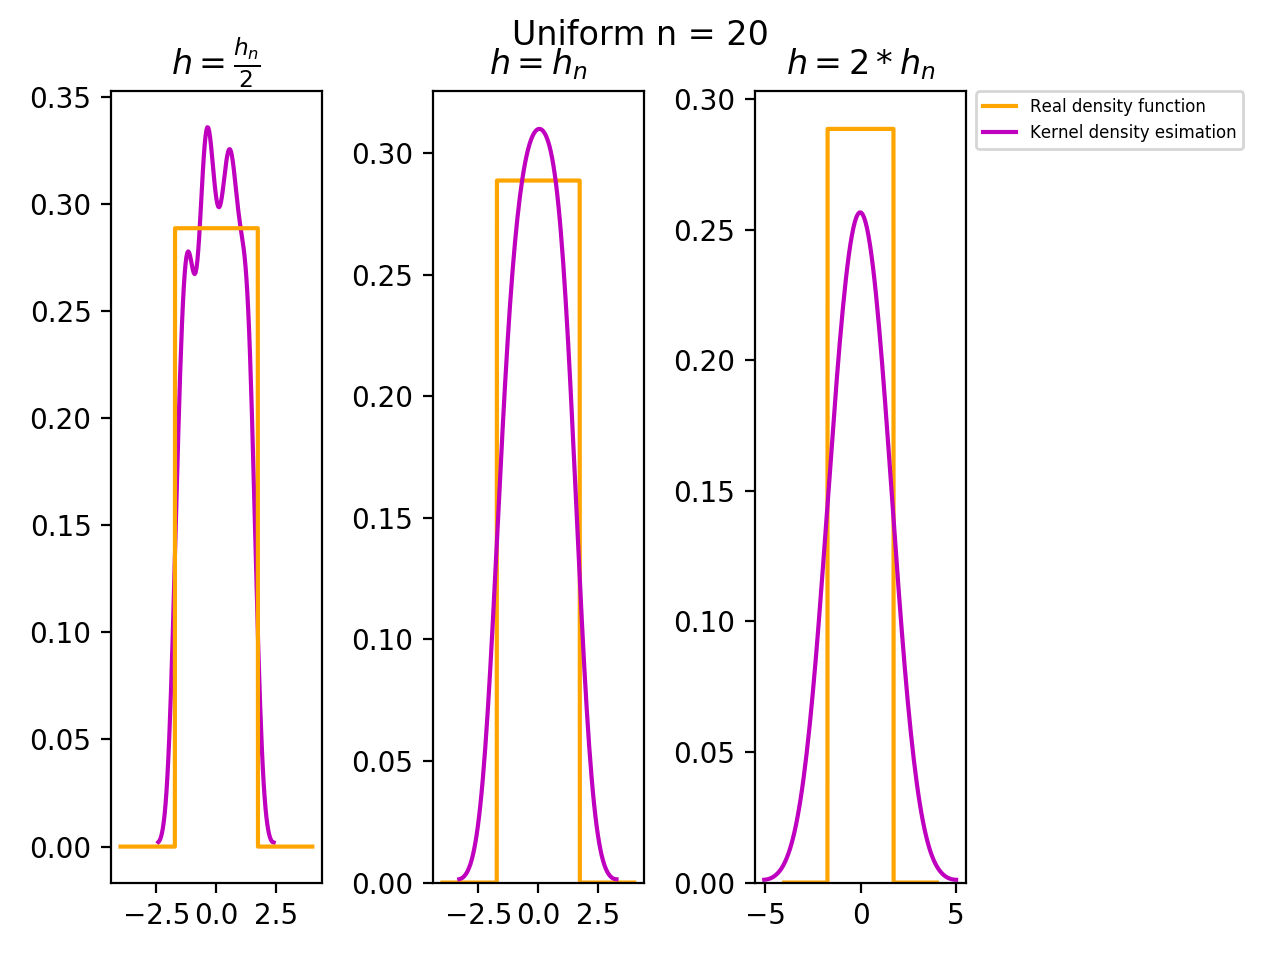
\includegraphics[scale=0.7]{fig/Uniform20_kde.png}
		\caption{Равномерное распределение, n = 20} 
		\label{pic:pic_name}
	\end{center}
\end{figure}

\begin{figure}[H]
	\begin{center}
		\includegraphics[scale=0.7]{fig/Uniform60_kde.png}
		\caption{Равномерное распределение, n = 60} 
		\label{pic:pic_name}
	\end{center}
\end{figure}

\begin{figure}[H]
	\begin{center}
		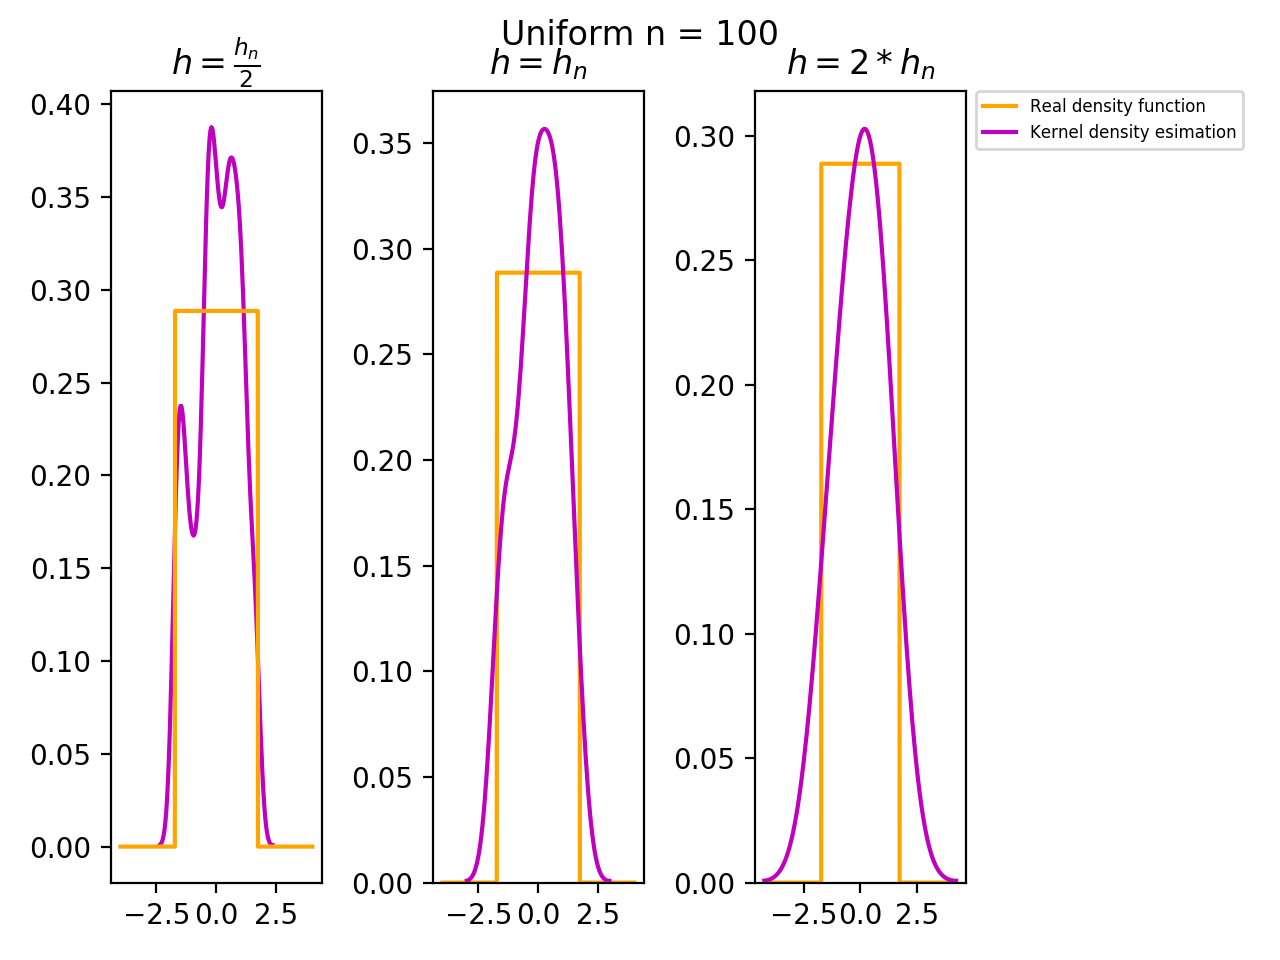
\includegraphics[scale=0.7]{fig/Uniform100_kde.png}
		\caption{Равномерное распределение, n = 100} 
		\label{pic:pic_name}
	\end{center}
\end{figure}


\section{Обсуждение}
Отметим, что чем больше выборка тем лучше полученные эмпирические функции функции распределения приближают теоретическую функцию распределения.
\\
Аналогично и с ядерной оценкой плотности - чем больше выборка, тем более приближенной к теоретической функции плотности распределения получается оценка.
\\
Также, сравнивали графики ядерной оценки плотности для различных диапазонов частот. Судя по графикам, можно заключить, что наилучшее приближение реализовано при выборе данного параметра по правилу Сильвермана. При увеличении и уменьшении данного значения приближение становится хуже. 


\section{Литература}
Максимов Ю. Д. Математическая статистика //СПб.: СПбГПУ. – 2004.

Гурский Е. И. Теория вероятностей с элементами математической статистики. – Высш. школа, 1971.

\section{Приложения}

Репозиторий с кодом программы и кодом отчёта: \href{https://github.com/unjamini/math-stat-lab}{https://github.com/unjamini/math-stat-lab}



